\documentclass[10pt,a4paper]{article}
\usepackage[latin1]{inputenc}
\usepackage{amsmath}
\usepackage{amsfonts}
\usepackage{amssymb}
\usepackage{graphicx}
\usepackage{subcaption}
\usepackage{pdfpages}
\usepackage[left=2.00cm, right=2.00cm, top=2.00cm, bottom=2.00cm]{geometry}
\begin{document}
	     \begin{center}
	 	\Large{\underline{\bf Methods Attempted}}
	 \end{center}
 
 \section{Original Report Method}
 We wish to find the probability of moving from a graph \(G\) to any other graph \(G'\) in the space of all graphs on \(n\) nodes, \(\mathcal{G}\), that is \(\mathbb{P}(G'|G)\). We can do this by using the Law of Total Probability, and partitioning the space by counting how many edge swaps are required to get from \(G\) to \(G'\). We will denote this \(\delta\).\par 
 We restrict our possible moves as follows:
 \[\mathbb{P}(G'|G) = \begin{cases}
 f(G,\delta) & \text{if }G' \text{ is within } \delta \text{ edge swaps of }G\\
 0
 & \text{otherwise}
 \end{cases}\]
 We define the set of all graphs within \(\delta\) edge swaps of \(G\) to be the \(\delta\)-neighbourhood of \(G\), denoted \(\mathrm{nbhd}_{\delta}(G)\). \par 
 If we restrict our choice of \(\delta\) to an interval \(\left[ -W/2,W/2\right]\backslash\{0\}\), we obtain
 \begin{align*}
 \mathbb{P}(G'|G)= \sum_{\substack{d=-W/2,\\ d\neq0}}^{W/2}\mathbb{P}(G'|G,\delta=d)\mathbb{P}(\delta=d)
 \end{align*}
 This can be calculated explicitly for \(W=2\).
 \begin{align*}
 \mathbb{P}(G'|G,\delta=-1) = \frac{\binom{m}{1}}{\binom{\binom{n}{2}}{m}}
 \end{align*}
 There are \(m\) possible edges to remove, of which we are choosing 1. This is divided by the number of graphs with \(m\) edges on \(n\) nodes. Similarly, 
  \begin{align*}
 \mathbb{P}(G'|G,\delta=1) = \frac{\binom{\binom{n}{2}-m}{1}}{\binom{\binom{n}{2}}{m}}
 \end{align*}
 Assigning a discrete uniform distribution on \(\delta\) gives \(\mathbb{P}(\delta=d)=\frac{1}{W}=\frac{1}{2}\). As such,
 \[\mathbb{P}(G'|G) = \frac{\binom{n}{2}}{2\binom{\binom{n}{2}}{m}}\]
 To extend to larger windows, I thought it would be the same, however choosing different numbers of links in the numerator.
 \begin{align*}
 q(G,G')=\frac{1}{W\binom{\binom{n}{2}}{m}}\left[\sum_{d=1}^{W/2} \binom{m}{d}+\binom{\binom{n}{2}-m}{d}\right]
 \end{align*} However, this fails even for \(W=4\), as it gives a probability greater than 1. I think the error lies in the denominator, as it remains constant while the numerator grows with every increase in window size. Using this in the algorithm clearly does not work, no proposals are accepted.

  \section{Report Code}
  In the algorithm, this was coded erroneously. The rejection step was inverted, i.e. \(\Delta Q(G,G') = -\log q(G,G')+\log q(G',G)\). When running this with \(n=100, p=0.01\) for \(10^6\) iterations, convergence is good. The Kolmogorov-Smirnov statistic is 0.0163. Figure \ref{fig:goodhist} shows a histogram comparison and a QQ plot.
  \begin{figure}[h]
  	\centering
  	\begin{subfigure}{\textwidth}
  		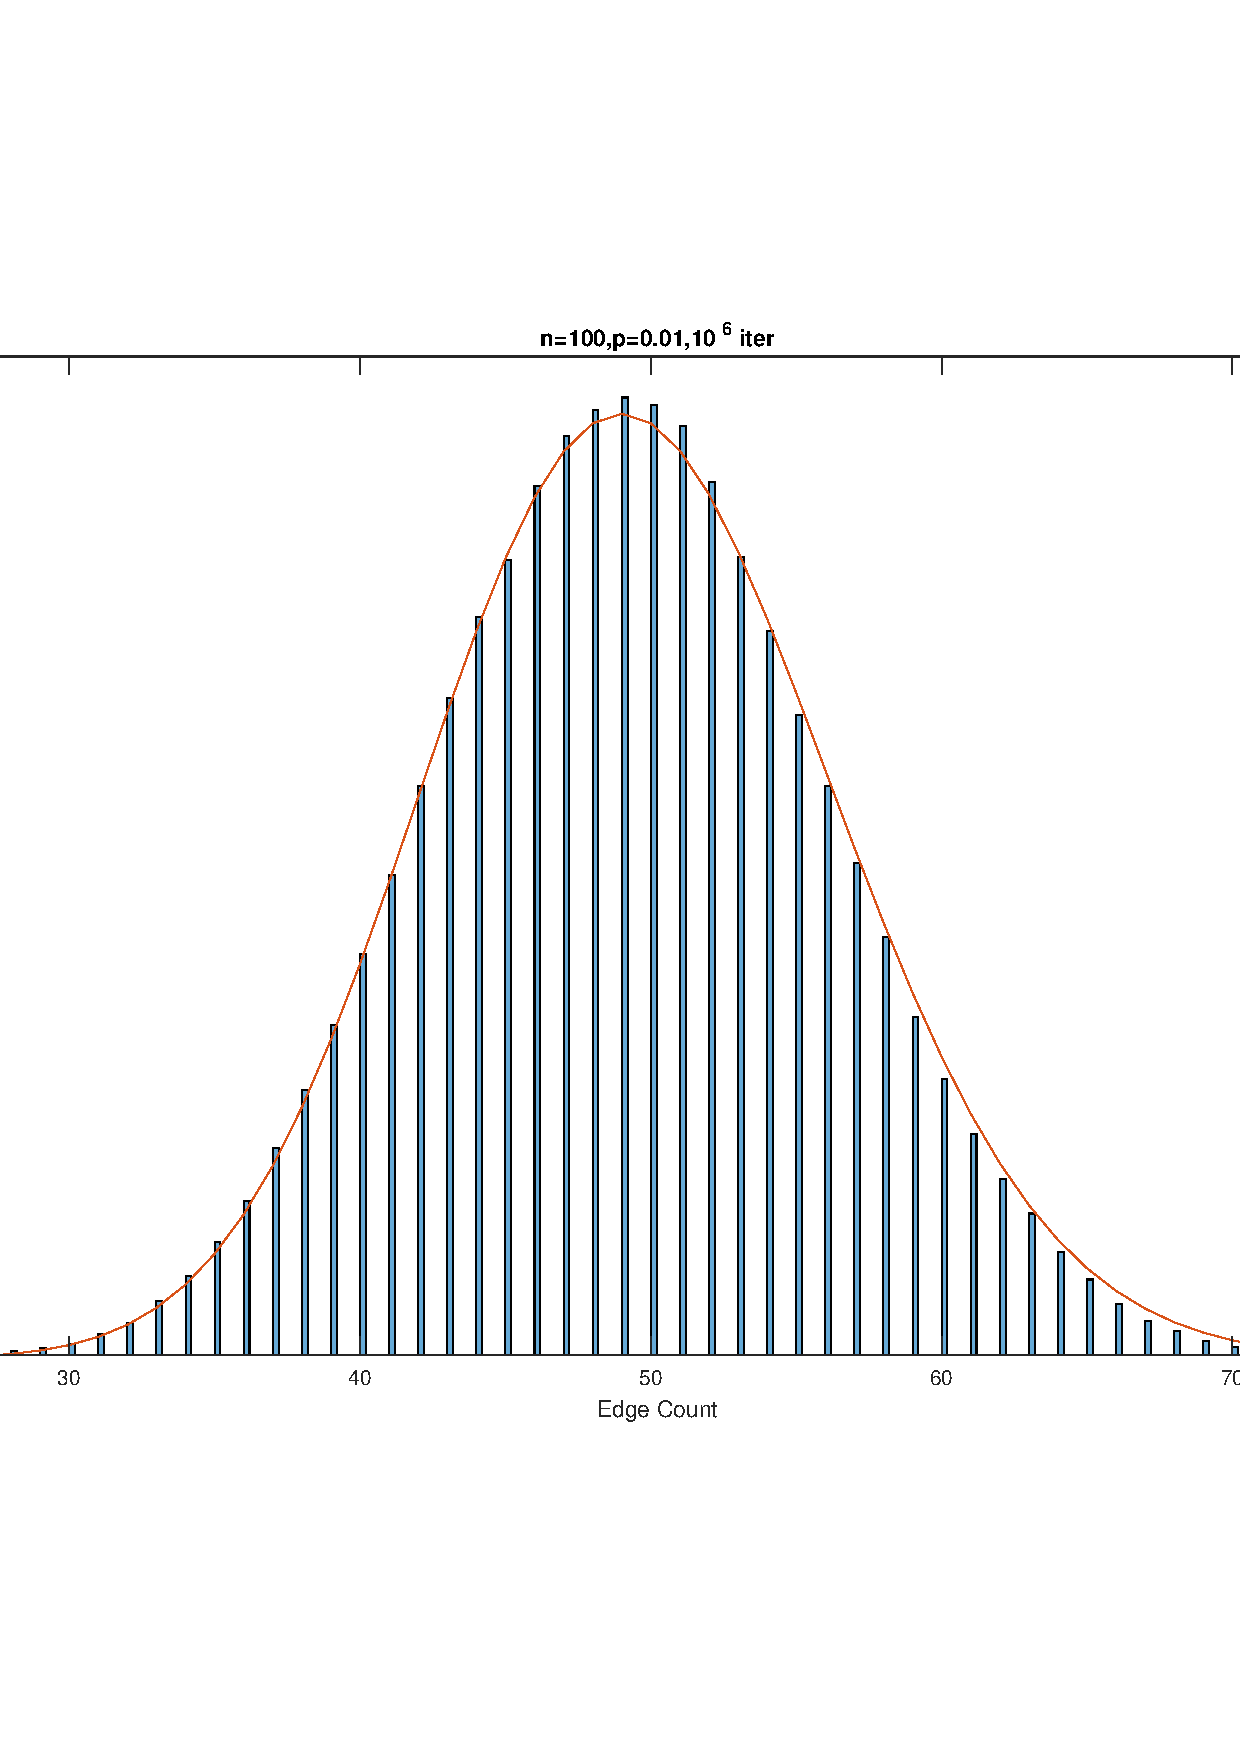
\includegraphics[width=\textwidth]{histogram}
  	\end{subfigure}\\%
  	\begin{subfigure}{\textwidth}
	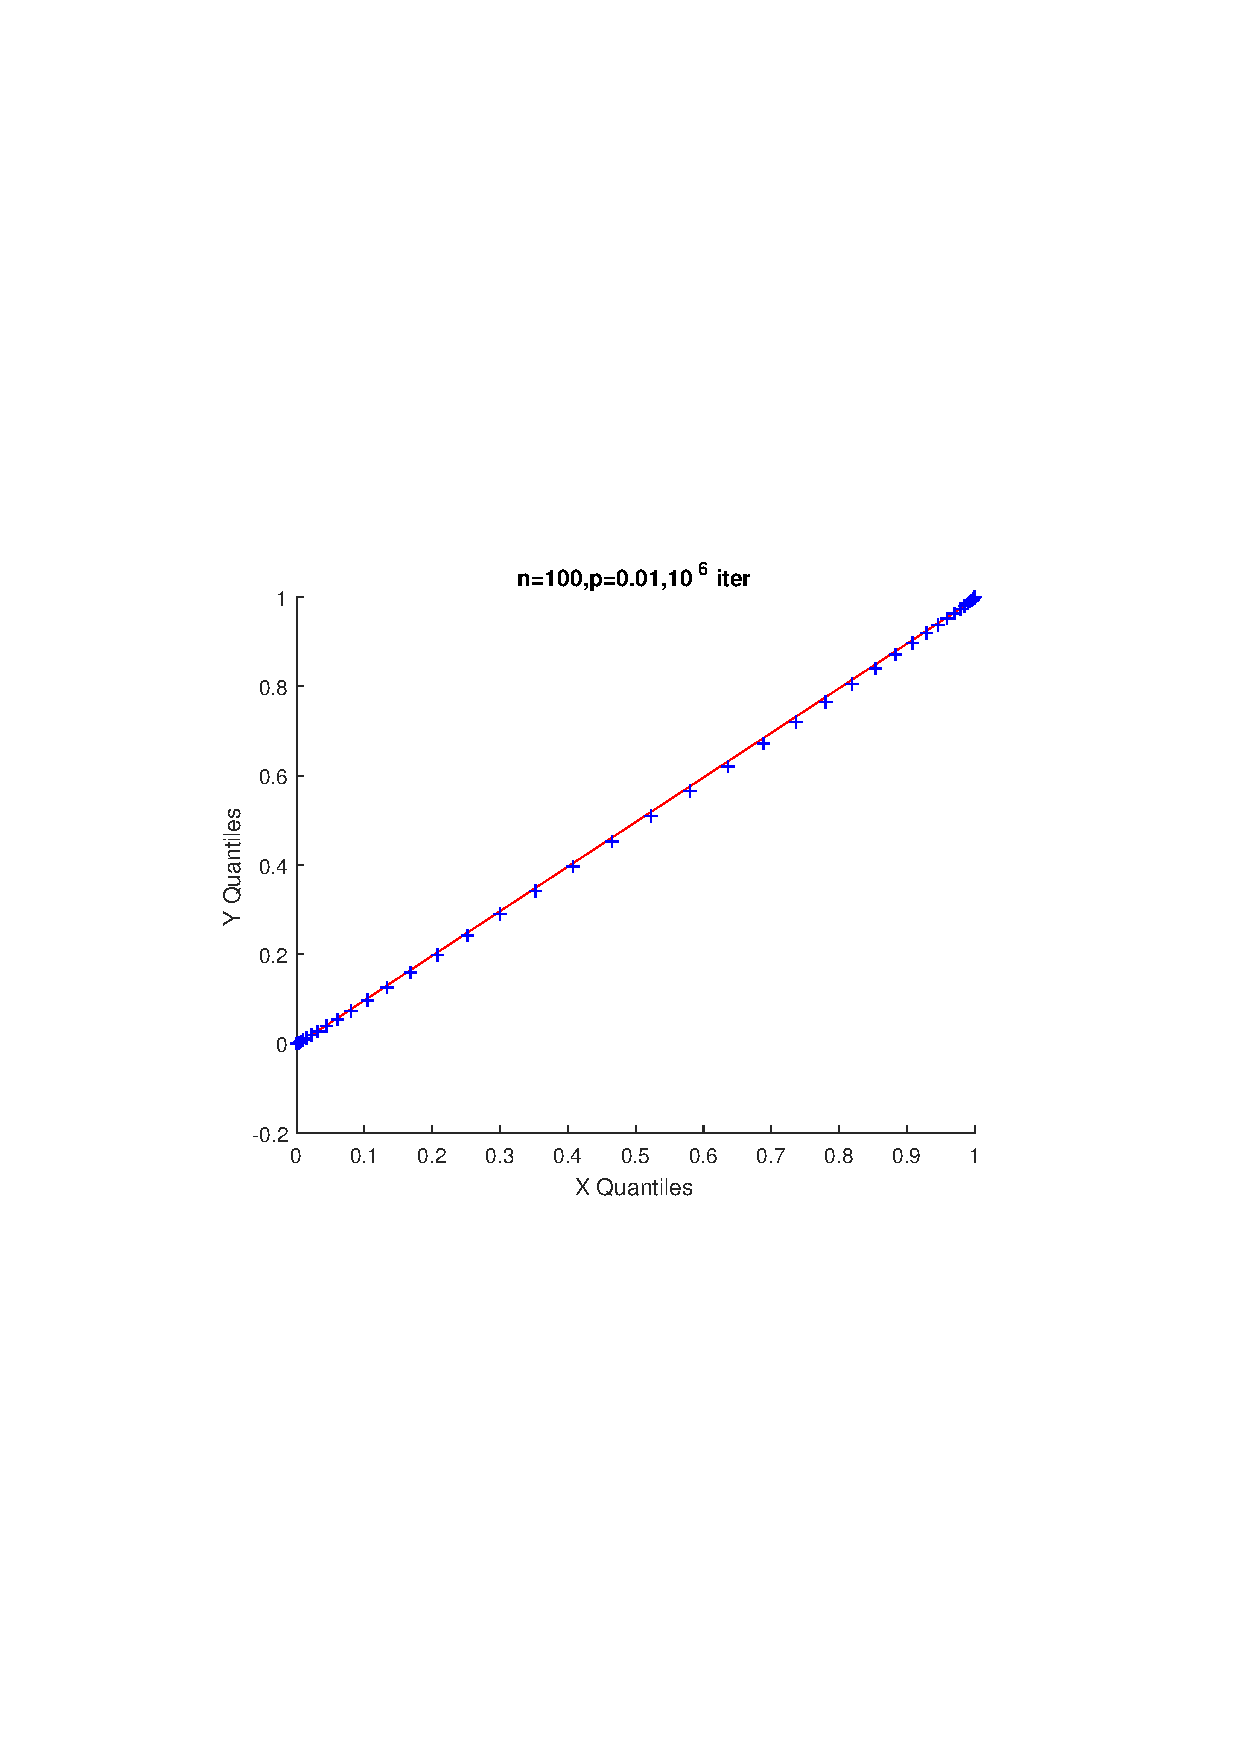
\includegraphics[width=\textwidth]{qq}
\end{subfigure}
\caption{Good Convergence for 100 nodes, 0.01 link density}
\label{fig:goodhist}
  \end{figure}
  \begin{figure}[h]\label{fig:ksstat}
	\centering
		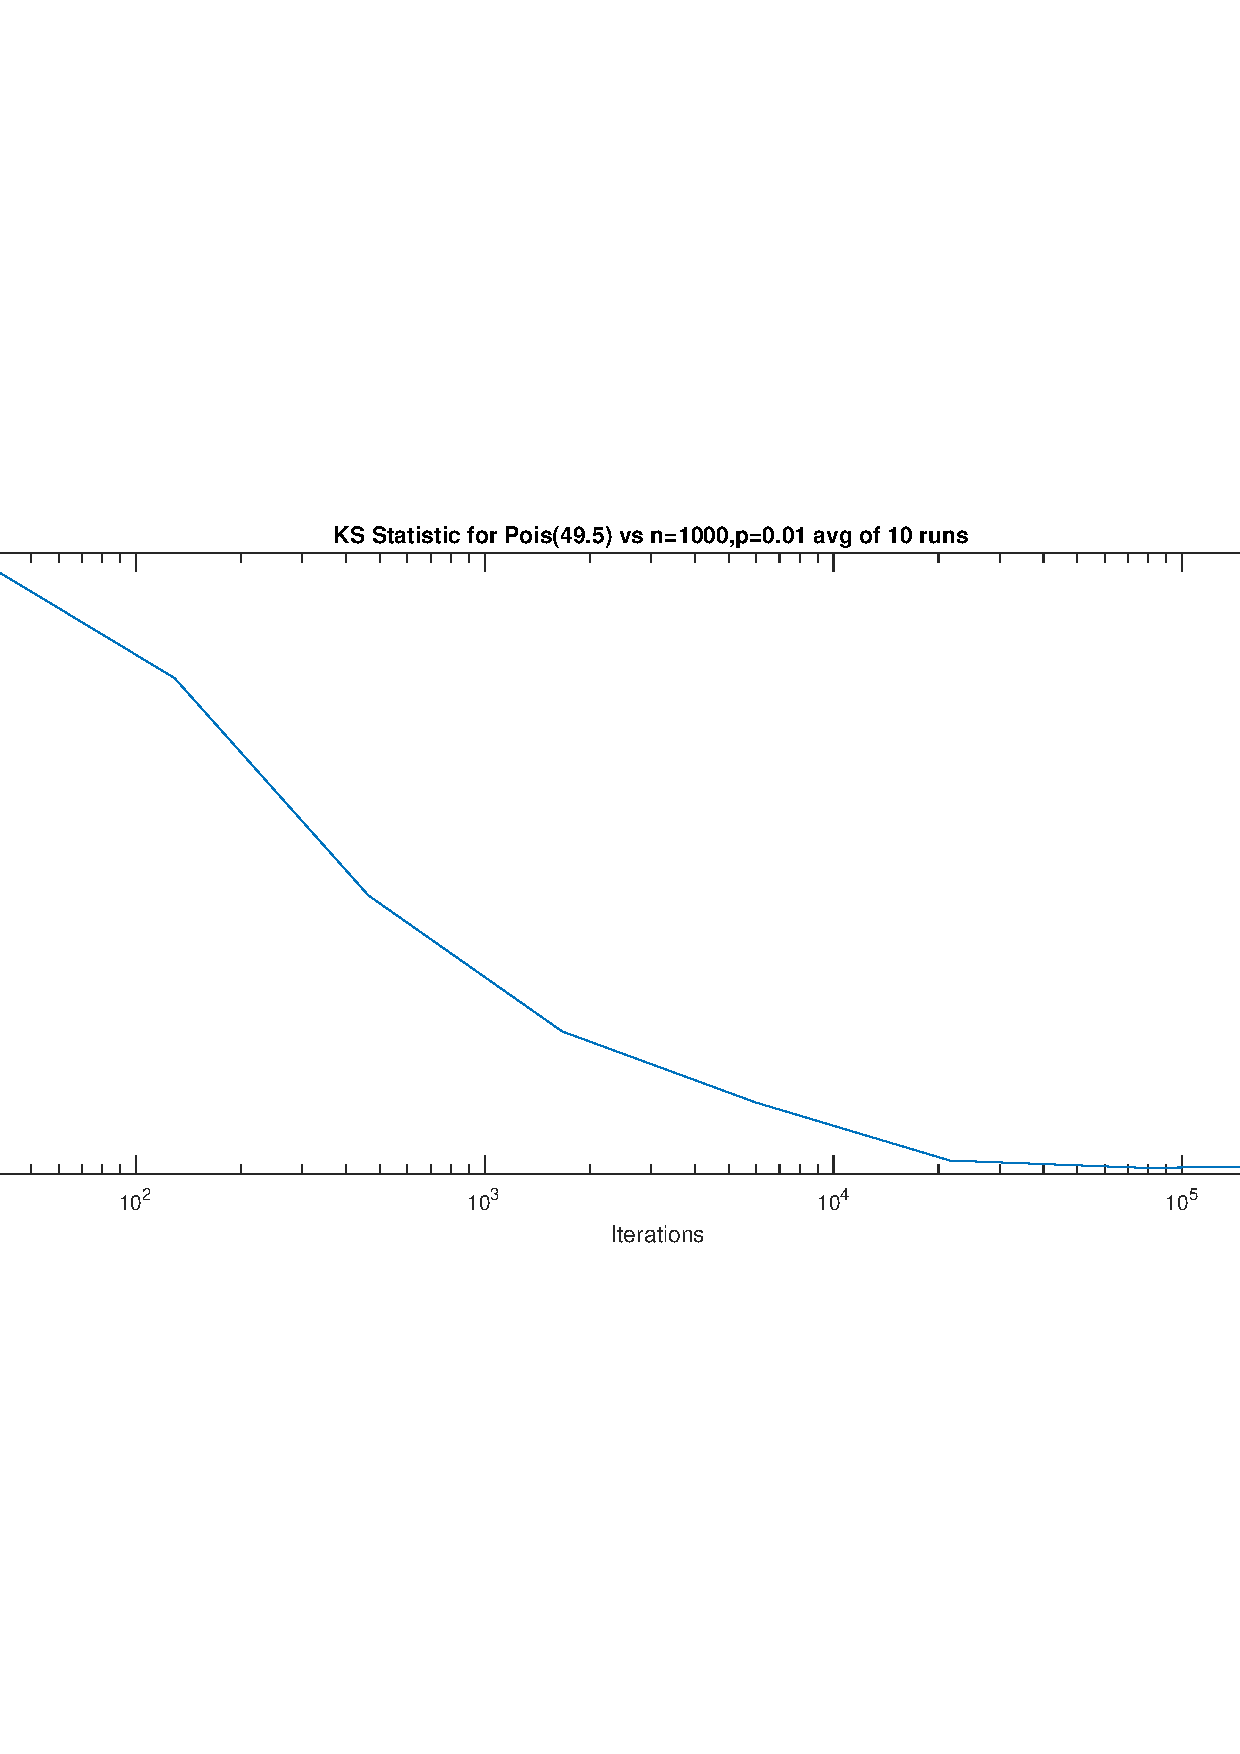
\includegraphics[width=\textwidth]{ksstat}
	\caption{KS Stat varying runtime 100 nodes, 0.01 link density}

\end{figure}

For n=1000, p=0.01: KS: 0.2824. Mean should be 4995. 

	\begin{figure}[h]
		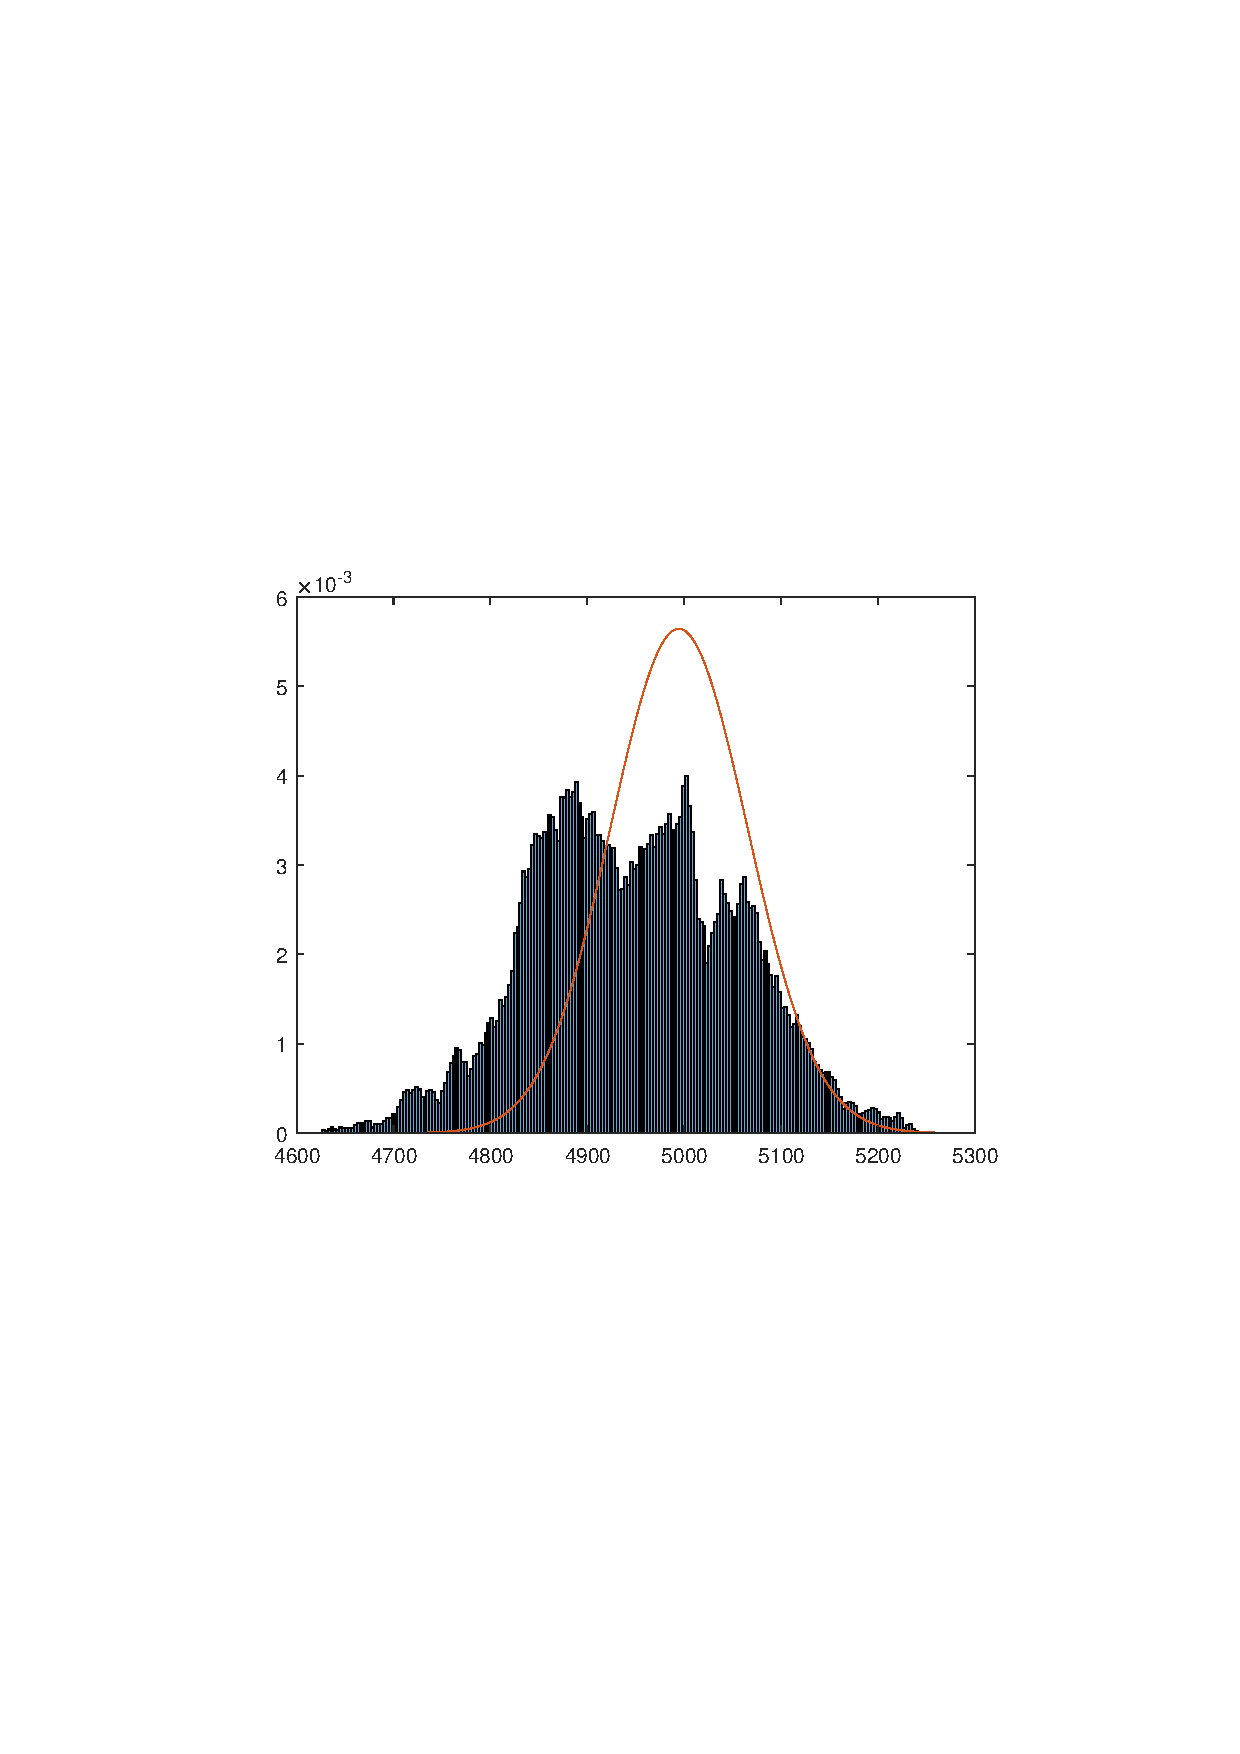
\includegraphics[width=\textwidth]{badhist}
	\end{figure}
	\begin{figure}[h]
		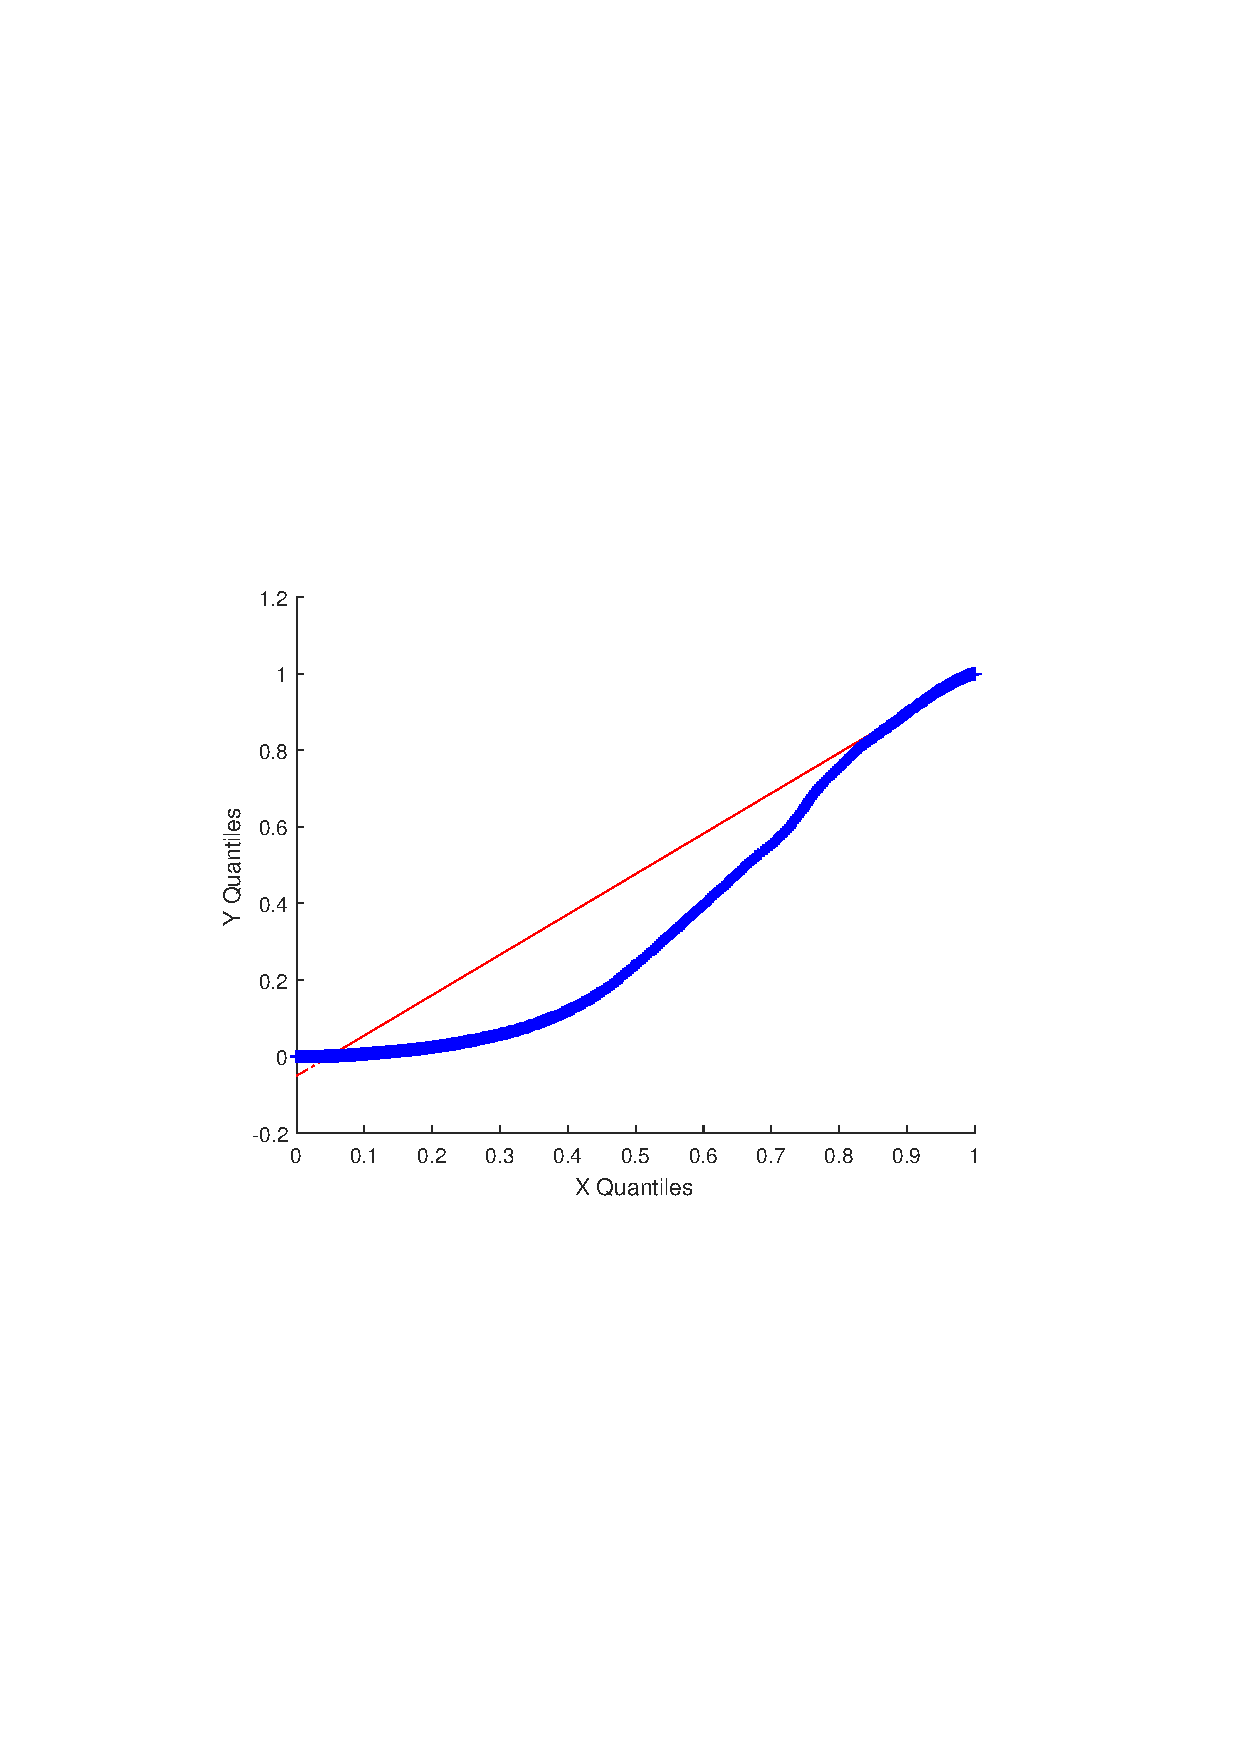
\includegraphics[width=\textwidth]{qqbad}
			\caption{Bad Convergence for 1000 nodes, 0.01 link density}
		\label{fig:badhist}
	\end{figure}



 \section{Discrete uniform over entire Graph space}
 Suggests \(\mathbb{P}(G'|G) = \frac{\mathbb{P}(\delta=m'-m)}{|\text{nbhd}_{\delta}G|}\) - also doesn't work
 \section{Difference in  m,m'}
 Not yet coded. Current best guess
 
\end{document}